\documentclass{standalone}
\usepackage{tikz}
\usetikzlibrary{patterns, positioning}

\begin{document}
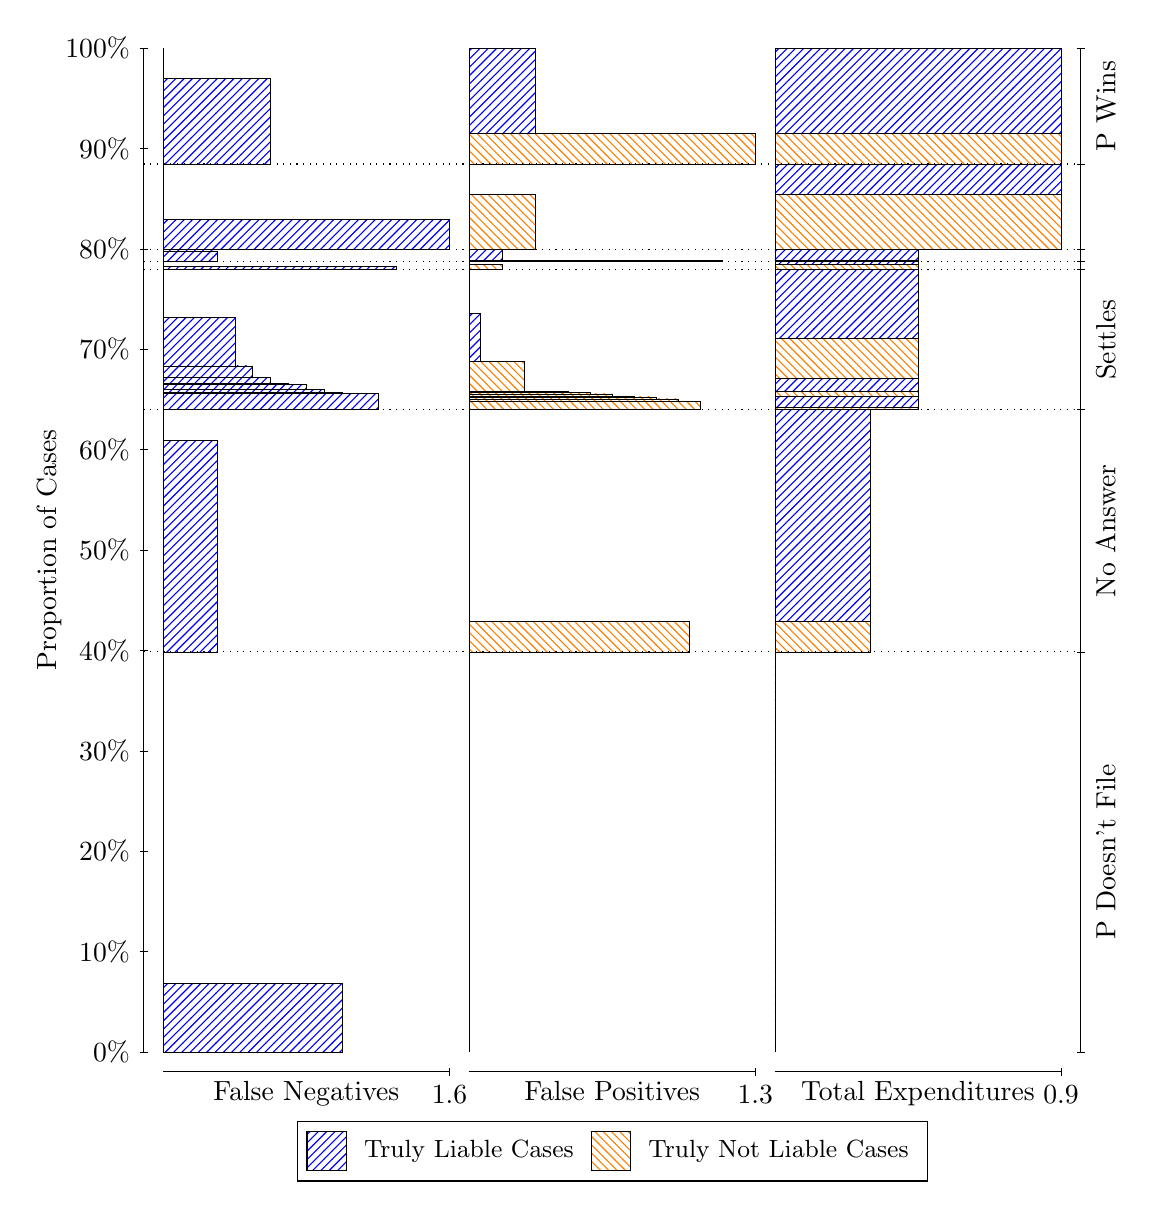
\begin{tikzpicture}
\draw[black, very thin] (1.5,1.75) -- (1.5,14.5);
\node[rotate=90, anchor=center] at (0.3, 8.125) {Proportion of Cases};
\draw[black, very thin] (1.45,1.75) -- (1.55,1.75);
\node[anchor=east] at (1.45, 1.75) {0\%};
\draw[black, very thin] (1.45,3.025) -- (1.55,3.025);
\node[anchor=east] at (1.45, 3.025) {10\%};
\draw[black, very thin] (1.45,4.3) -- (1.55,4.3);
\node[anchor=east] at (1.45, 4.3) {20\%};
\draw[black, very thin] (1.45,5.575) -- (1.55,5.575);
\node[anchor=east] at (1.45, 5.575) {30\%};
\draw[black, very thin] (1.45,6.85) -- (1.55,6.85);
\node[anchor=east] at (1.45, 6.85) {40\%};
\draw[black, very thin] (1.45,8.125) -- (1.55,8.125);
\node[anchor=east] at (1.45, 8.125) {50\%};
\draw[black, very thin] (1.45,9.4) -- (1.55,9.4);
\node[anchor=east] at (1.45, 9.4) {60\%};
\draw[black, very thin] (1.45,10.675) -- (1.55,10.675);
\node[anchor=east] at (1.45, 10.675) {70\%};
\draw[black, very thin] (1.45,11.95) -- (1.55,11.95);
\node[anchor=east] at (1.45, 11.95) {80\%};
\draw[black, very thin] (1.45,13.225) -- (1.55,13.225);
\node[anchor=east] at (1.45, 13.225) {90\%};
\draw[black, very thin] (1.45,14.5) -- (1.55,14.5);
\node[anchor=east] at (1.45, 14.5) {100\%};

\draw[black, very thin] (13.4,1.75) -- (13.4,14.5);
\draw[black, very thin] (13.35,1.75) -- (13.45,1.75);
\node[anchor=west] at (13.35, 1.75) {};
\draw[black, very thin] (13.35,6.8304) -- (13.45,6.8304);
\node[anchor=west] at (13.35, 6.8304) {};
\draw[black, very thin] (13.35,9.9066) -- (13.45,9.9066);
\node[anchor=west] at (13.35, 9.9066) {};
\draw[black, very thin] (13.35,11.69) -- (13.45,11.69);
\node[anchor=west] at (13.35, 11.69) {};
\draw[black, very thin] (13.35,11.786) -- (13.45,11.786);
\node[anchor=west] at (13.35, 11.786) {};
\draw[black, very thin] (13.35,11.943) -- (13.45,11.943);
\node[anchor=west] at (13.35, 11.943) {};
\draw[black, very thin] (13.35,13.027) -- (13.45,13.027);
\node[anchor=west] at (13.35, 13.027) {};
\draw[black, very thin] (13.35,14.5) -- (13.45,14.5);
\node[anchor=west] at (13.35, 14.5) {};

\draw[black, very thin, pattern color=blue, pattern=north east lines] (1.75,1.75) rectangle (4.0208,2.6245);
\draw[black, very thin, pattern color=orange, pattern=north west lines] (1.75,2.6245) rectangle (1.75,6.8304);
\draw[black, very thin, pattern color=blue, pattern=north east lines] (1.75,6.8304) rectangle (2.4312,9.5137);
\draw[black, very thin, pattern color=orange, pattern=north west lines] (1.75,9.5137) rectangle (1.75,9.9066);
\draw[black, very thin, pattern color=blue, pattern=north east lines] (1.75,9.9066) rectangle (4.475,10.111);
\draw[black, very thin, pattern color=blue, pattern=north east lines] (1.75,10.111) rectangle (4.2479,10.118);
\draw[black, very thin, pattern color=blue, pattern=north east lines] (1.75,10.118) rectangle (4.0208,10.13);
\draw[black, very thin, pattern color=blue, pattern=north east lines] (1.75,10.13) rectangle (3.7937,10.162);
\draw[black, very thin, pattern color=blue, pattern=north east lines] (1.75,10.162) rectangle (3.7937,10.163);
\draw[black, very thin, pattern color=blue, pattern=north east lines] (1.75,10.163) rectangle (3.5667,10.232);
\draw[black, very thin, pattern color=blue, pattern=north east lines] (1.75,10.232) rectangle (3.3396,10.242);
\draw[black, very thin, pattern color=blue, pattern=north east lines] (1.75,10.242) rectangle (3.1125,10.321);
\draw[black, very thin, pattern color=blue, pattern=north east lines] (1.75,10.321) rectangle (2.8854,10.464);
\draw[black, very thin, pattern color=blue, pattern=north east lines] (1.75,10.464) rectangle (2.6583,11.079);
\draw[black, very thin, pattern color=orange, pattern=north west lines] (1.75,11.079) rectangle (1.75,11.69);
\draw[black, very thin, pattern color=blue, pattern=north east lines] (1.75,11.69) rectangle (4.7021,11.725);
\draw[black, very thin, pattern color=orange, pattern=north west lines] (1.75,11.725) rectangle (1.75,11.786);
\draw[black, very thin, pattern color=blue, pattern=north east lines] (1.75,11.786) rectangle (2.4312,11.925);
\draw[black, very thin, pattern color=orange, pattern=north west lines] (1.75,11.925) rectangle (1.75,11.943);
\draw[black, very thin, pattern color=blue, pattern=north east lines] (1.75,11.943) rectangle (5.3833,12.326);
\draw[black, very thin, pattern color=orange, pattern=north west lines] (1.75,12.326) rectangle (1.75,13.027);
\draw[black, very thin, pattern color=blue, pattern=north east lines] (1.75,13.027) rectangle (3.1125,14.115);
\draw[black, very thin, pattern color=orange, pattern=north west lines] (1.75,14.115) rectangle (1.75,14.5);
\draw[black, very thin, pattern color=orange, pattern=north west lines] (5.6333,1.75) rectangle (5.6333,5.9559);
\draw[black, very thin, pattern color=blue, pattern=north east lines] (5.6333,5.9559) rectangle (5.6333,6.8304);
\draw[black, very thin, pattern color=orange, pattern=north west lines] (5.6333,6.8304) rectangle (8.4282,7.2233);
\draw[black, very thin, pattern color=blue, pattern=north east lines] (5.6333,7.2233) rectangle (5.6333,9.9066);
\draw[black, very thin, pattern color=orange, pattern=north west lines] (5.6333,9.9066) rectangle (8.5679,10.014);
\draw[black, very thin, pattern color=orange, pattern=north west lines] (5.6333,10.014) rectangle (8.2885,10.043);
\draw[black, very thin, pattern color=orange, pattern=north west lines] (5.6333,10.043) rectangle (8.009,10.069);
\draw[black, very thin, pattern color=orange, pattern=north west lines] (5.6333,10.069) rectangle (7.7295,10.076);
\draw[black, very thin, pattern color=orange, pattern=north west lines] (5.6333,10.076) rectangle (7.45,10.107);
\draw[black, very thin, pattern color=orange, pattern=north west lines] (5.6333,10.107) rectangle (7.1705,10.107);
\draw[black, very thin, pattern color=orange, pattern=north west lines] (5.6333,10.107) rectangle (7.1705,10.129);
\draw[black, very thin, pattern color=orange, pattern=north west lines] (5.6333,10.129) rectangle (6.891,10.138);
\draw[black, very thin, pattern color=orange, pattern=north west lines] (5.6333,10.138) rectangle (6.6115,10.142);
\draw[black, very thin, pattern color=orange, pattern=north west lines] (5.6333,10.142) rectangle (6.3321,10.518);
\draw[black, very thin, pattern color=blue, pattern=north east lines] (5.6333,10.518) rectangle (5.7731,11.133);
\draw[black, very thin, pattern color=blue, pattern=north east lines] (5.6333,11.133) rectangle (5.6333,11.69);
\draw[black, very thin, pattern color=orange, pattern=north west lines] (5.6333,11.69) rectangle (6.0526,11.752);
\draw[black, very thin, pattern color=blue, pattern=north east lines] (5.6333,11.752) rectangle (5.6333,11.786);
\draw[black, very thin, pattern color=orange, pattern=north west lines] (5.6333,11.786) rectangle (8.8474,11.804);
\draw[black, very thin, pattern color=blue, pattern=north east lines] (5.6333,11.804) rectangle (6.0526,11.943);
\draw[black, very thin, pattern color=orange, pattern=north west lines] (5.6333,11.943) rectangle (6.4718,12.644);
\draw[black, very thin, pattern color=blue, pattern=north east lines] (5.6333,12.644) rectangle (5.6333,13.027);
\draw[black, very thin, pattern color=orange, pattern=north west lines] (5.6333,13.027) rectangle (9.2667,13.412);
\draw[black, very thin, pattern color=blue, pattern=north east lines] (5.6333,13.412) rectangle (6.4718,14.5);
\draw[black, very thin, pattern color=orange, pattern=north west lines] (9.5167,1.75) rectangle (9.5167,5.9559);
\draw[black, very thin, pattern color=blue, pattern=north east lines] (9.5167,5.9559) rectangle (9.5167,6.8304);
\draw[black, very thin, pattern color=orange, pattern=north west lines] (9.5167,6.8304) rectangle (10.728,7.2233);
\draw[black, very thin, pattern color=blue, pattern=north east lines] (9.5167,7.2233) rectangle (10.728,9.9066);
\draw[black, very thin, pattern color=orange, pattern=north west lines] (9.5167,9.9066) rectangle (11.333,9.936);
\draw[black, very thin, pattern color=blue, pattern=north east lines] (9.5167,9.936) rectangle (11.333,10.08);
\draw[black, very thin, pattern color=orange, pattern=north west lines] (9.5167,10.08) rectangle (11.333,10.143);
\draw[black, very thin, pattern color=blue, pattern=north east lines] (9.5167,10.143) rectangle (11.333,10.302);
\draw[black, very thin, pattern color=orange, pattern=north west lines] (9.5167,10.302) rectangle (11.333,10.82);
\draw[black, very thin, pattern color=blue, pattern=north east lines] (9.5167,10.82) rectangle (11.333,11.69);
\draw[black, very thin, pattern color=orange, pattern=north west lines] (9.5167,11.69) rectangle (11.333,11.752);
\draw[black, very thin, pattern color=blue, pattern=north east lines] (9.5167,11.752) rectangle (11.333,11.786);
\draw[black, very thin, pattern color=orange, pattern=north west lines] (9.5167,11.786) rectangle (11.333,11.804);
\draw[black, very thin, pattern color=blue, pattern=north east lines] (9.5167,11.804) rectangle (11.333,11.943);
\draw[black, very thin, pattern color=orange, pattern=north west lines] (9.5167,11.943) rectangle (13.15,12.644);
\draw[black, very thin, pattern color=blue, pattern=north east lines] (9.5167,12.644) rectangle (13.15,13.027);
\draw[black, very thin, pattern color=orange, pattern=north west lines] (9.5167,13.027) rectangle (13.15,13.412);
\draw[black, very thin, pattern color=blue, pattern=north east lines] (9.5167,13.412) rectangle (13.15,14.5);
\draw[black, dotted] (1.5,6.8304) -- (13.4,6.8304);
\draw[black, dotted] (1.5,9.9066) -- (13.4,9.9066);
\draw[black, dotted] (1.5,11.69) -- (13.4,11.69);
\draw[black, dotted] (1.5,11.786) -- (13.4,11.786);
\draw[black, dotted] (1.5,11.943) -- (13.4,11.943);
\draw[black, dotted] (1.5,13.027) -- (13.4,13.027);
\draw[black, very thin] (1.75,1.5) -- (5.3833,1.5);
\node[anchor=north] at (3.5667, 1.5) {False Negatives};
\draw[black, very thin] (5.3833,1.45) -- (5.3833,1.55);
\node[anchor=north] at (5.3833, 1.45) {1.6};

\draw[black, very thin] (5.6333,1.5) -- (9.2667,1.5);
\node[anchor=north] at (7.45, 1.5) {False Positives};
\draw[black, very thin] (9.2667,1.45) -- (9.2667,1.55);
\node[anchor=north] at (9.2667, 1.45) {1.3};

\draw[black, very thin] (9.5167,1.5) -- (13.15,1.5);
\node[anchor=north] at (11.333, 1.5) {Total Expenditures};
\draw[black, very thin] (13.15,1.45) -- (13.15,1.55);
\node[anchor=north] at (13.15, 1.45) {0.9};

\node[black, centered, rotate=90] at (13.72, 4.2902) {P Doesn't File};
\node[black, centered, rotate=90] at (13.72, 8.3685) {No Answer};
\node[black, centered, rotate=90] at (13.72, 10.799) {Settles};



\node[black, centered, rotate=90] at (13.72, 13.763) {P Wins};

\draw (7.449999999999999,1.5) node[draw=none] (baseCoordinate) {};
\begin{scope}[align=center]
        \matrix[scale=0.5, draw=black, below=0.5cm of baseCoordinate, nodes={draw}, column sep=0.1cm]{
            \node[rectangle, draw, minimum width=0.5cm, minimum height=0.5cm, pattern=north east lines, pattern color=blue] {}; &
            \node[draw=none, font=\small] (B) {Truly Liable Cases}; &
            \node[rectangle, draw, minimum width=0.5cm, minimum height=0.5cm, pattern=north west lines, pattern color=orange] {}; &
            \node[draw=none, font=\small] (B) {Truly Not Liable Cases}; \\
            };
\end{scope}

\end{tikzpicture}
\end{document}